\documentclass[convert]{standalone}

\usepackage{tikz}
\usepackage{graphicx}
\pagestyle{empty}

% INT_AY22_L28-Fig06_Two_amp_loops.png

\begin{document}
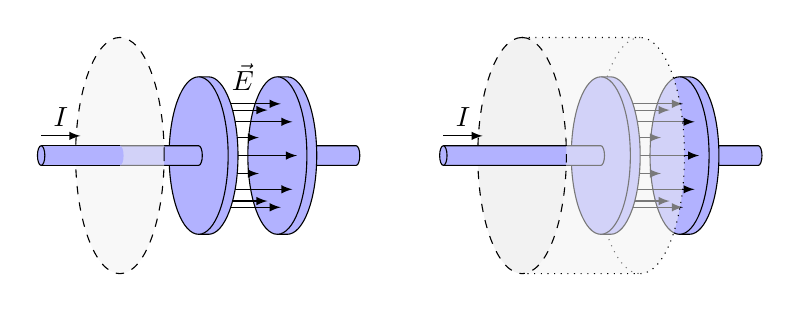
\begin{tikzpicture}[> = latex]

\matrix[column sep = 1 cm]{
	
	% Wire to right of right plate
	
	\draw [fill = blue!30] (2, 0.125) -- (3, 0.125) arc (90 : -90 : 0.0469 and 0.125) -- (2, -0.125);

	% Capacitor plates + electric field
	
	\draw [fill = blue!30] (2, 1) -- (2.125, 1) arc (90 : -90 : 0.375 and 1) -- (2, -1);
	\draw [fill = blue!30] (2, 0) ellipse (0.375 and 1);
	
	\node at (1.5625, 1) {${\vec E}$};
	\foreach \Q in {0, 40, ..., 320}
		\draw [->] ({1 + 0.25 * cos(\Q)}, {0.667 * sin(\Q)}) -- ({2 + 0.25 * cos(\Q)}, {0.667 * sin(\Q)});
	
	\draw [fill = blue!30] (1, 1) -- (1.125, 1) arc (90 : -90 : 0.375 and 1) -- (1, -1);
	\draw [fill = blue!30] (1, 0) ellipse (0.375 and 1);
	
	% Wire between loop and left plate
	
	\draw [fill = blue!30] (0, 0.125) -- (1, 0.125) arc (90 : -90 : 0.0469 and 0.125) -- (0, -0.125);
	
	% Amperian loop
	
	\draw [draw = none, fill = gray!10, opacity = 0.5] (0, 0) ellipse (0.5625 and 1.5);
	\draw [dashed] (0, 0) ellipse (0.5625 and 1.5);
	
	% Wire to left to loop
	
	\draw [fill = blue!30, draw = none] (-1, 0.125) -- (0, 0.125) arc (90 : -90 : 0.0469 and 0.125) -- (-1, -0.125);
	\draw (-1, 0.125) -- (0, 0.125);
	\draw (-1, -0.125) -- (0, -0.125);
	
	\draw [fill = blue!30] (-1, 0) ellipse (0.0469 and 0.125);
	
	% Current arrow
	
	\draw [->] (-1, 0.25) -- node [above] {$I$} (-0.5, 0.25);
	
&

	% Indicator for right face of area cylinder

	\draw [dotted] (1.5, 1.5) arc (90 : 270 : 0.5625 and 1.5);
	
	% Wire to right of right plate
	
	\draw [fill = blue!30] (2, 0.125) -- (3, 0.125) arc (90 : -90 : 0.0469 and 0.125) -- (2, -0.125);

	% Capacitor plates + electric field
	
	\draw [fill = blue!30] (2, 1) -- (2.125, 1) arc (90 : -90 : 0.375 and 1) -- (2, -1);
	\draw [fill = blue!30] (2, 0) ellipse (0.375 and 1);
	
	\foreach \Q in {0, 40, ..., 320}
		\draw [->] ({1 + 0.25 * cos(\Q)}, {0.667 * sin(\Q)}) -- ({2 + 0.25 * cos(\Q)}, {0.667 * sin(\Q)});
	
	\draw [fill = blue!30] (1, 1) -- (1.125, 1) arc (90 : -90 : 0.375 and 1) -- (1, -1);
	\draw [fill = blue!30] (1, 0) ellipse (0.375 and 1);
	
	% Amperian loop (part 1)
	
	\draw [dashed, fill = gray!10] (0, 1.5) arc (90 : 270 : 0.5625 and 1.5);
	\draw [draw = none, fill = gray!10] (0, 1.5) arc (90 : -90 : 0.5625 and 1.5) -- cycle;
	
	% Wire to left plate
	
	\draw [fill = blue!30] (-1, 0.125) -- (1, 0.125) arc (90 : -90 : 0.0469 and 0.125) -- (-1, -0.125);
	\draw [fill = blue!30] (-1, 0) ellipse (0.0469 and 0.125);
	
	% Current arrow
	
	\draw [->] (-1, 0.25) -- node [above] {$I$} (-0.5, 0.25);
	
	% Amperian loop (part 2)
	
	\draw [fill = gray!10, opacity = 0.5] (0, 1.5) -- (1.5, 1.5) arc (90 : -90 : 0.5625 and 1.5) -- (0, -1.5) [draw = none] arc (-90 : 90 : 0.5625 and 1.5);
	\draw [dashed] (0, 1.5) arc (90 : -90 : 0.5625 and 1.5);
	\draw [dotted] (0, 1.5) -- (1.5, 1.5) arc (90 : -90 : 0.5625 and 1.5) -- (0, -1.5);

\\
};

\end{tikzpicture}
\end{document}